

\section{Benchmarks and an Evaluation Process}

% \roni{Terminology discussion: so far we did not use the term ``operator''. Here we do. I think you mean here lifted action? if so, let's use the same terminology all over. I dislike operator as I can never remember if operator is the grounded version of the lifted one.}\leo{sure I replaced it with `lifted action`}

% \todo{Leonardo is in charge of this section.} Argaman also 

\begin{table}[ht]
\centering
\resizebox{\columnwidth}{!}{
\addtolength{\tabcolsep}{-0.2em}
    \centering
    \begin{tabular}{|l|c|c|c|c|c|c|c|c|c|c|}
    % \toprule
    \hline
    Domain & $|A|$ & $|P|$ & Types & Const. & \multicolumn{2}{c|}{$A$ arity} & \multicolumn{2}{c|}{$P$ arity} & Neg. & Inj. \\ 
     &  &  & & & $min$ & $max$ & $min$ & $max$ & pre.  & ass. \\ \hline
    % \midrule
barman & 12 & 15 & 9 & no & 2 & 6 & 1 & 2 & no & yes \\ %
blocksworld & 4 & 5 & 1 & no & 1 & 2 & 0 & 2 & no & yes \\ %
childsnack & 6 & 13 & 6 & yes & 2 & 4 & 1 & 2 & no & no \\ %
depots & 5 & 6 & 9 & no & 3 & 4 & 1 & 2 & no & yes \\ %
elevators & 6 & 8 & 5 & no & 3 & 5 & 2 & 2 & no & yes \\ %
ferry & 3 & 5 & 2 & no & 2 & 2 & 0 & 2 & no & yes \\ % 
floortile & 7 & 10 & 3 & no & 3 & 4 & 1 & 2 & no & yes \\ %
goldminer & 7 & 12 & 1 & no & 1 & 2 & 0 & 2 & yes & no \\ %
grippers & 3 & 4 & 4 & no & 3 & 4 & 2 & 3 & no & yes \\ %
matchingbw & 10 & 10 & 2 & no & 2 & 3 & 1 & 2 & yes & yes \\ %
miconic & 4 & 6 & 2 & no & 2 & 2 & 1 & 2 & no & yes \\ %
nomystery & 3 & 6 & 5 & no & 3 & 6 & 2 & 3 & no & yes \\ %
npuzzle & 1 & 3 & 2 & no & 3 & 3 & 1 & 2 & no & yes \\ %
parking & 4 & 5 & 2 & no & 3 & 3 & 1 & 2 & no & yes \\ %
rovers & 9 & 25 & 7 & no & 2 & 6 & 1 & 3 & no & no \\ %
satellite & 5 & 8 & 4 & no & 2 & 4 & 1 & 2 & yes & yes \\ %
sokoban & 2 & 4 & 3 & no & 3 & 5 & 1 & 3 & no & yes \\ %
spanner & 3 & 6 & 5 & no & 3 & 4 & 1 & 2 & no & yes \\ %
tpp & 4 & 7 & 7 & no & 3 & 7 & 2 & 3 & no & no \\ %
transport & 3 & 5 & 6 & no & 3 & 5 & 2 & 2 & no & yes \\ %
\hline

    % \hline
    \end{tabular}
    }
    \caption{Details about the benchmark domains that are relevant to domain model learning algorithms. The columns from left to right correspond to the name of the domain; the number of lifted actions, lifted predicates , and types; if there are constants; the min. and max. arity of the actions; the min. and max. arity of the predicates; if a literal can be a delete effects without being a preconditions; and if the 
    injective binding assumption holds~\citep{juba2021safe}, i.e., 
    whether a grounded action may map the same object to multiple parameters.}
    \label{tab:domains}
\end{table}


%\subsection{Benchmark}
Next, we describe a process for evaluating domain model learning algorithms 
and computing the metrics defined above. % and propose a corresponding set of domain model learning problems as a benchmark. 
% by experimenting with state-of-the-art approaches on a newly generated benchmark for offline learning of classical planning domains.
%
As a standard benchmark, we propose to use the set of $20$ classical planning domains used in all previous IPC learning tracks \citep{fern2011first, vallati20152014, taitler20242023}. 
These domains serve as both the environment and a reference domain model (for metrics that require one). 
We chose these domains for simplicity, as they are well known in the planning community. 
The number of lifted actions, predicates, and object types in these domains varies in 
$[1, 12]$, $[3,25]$, and $[1, 9]$, respectively.
Further details about the benchmark domains are provided in Table~\ref{tab:domains}. 

% \footnote{\label{foot:supplementary} Further details about the benchmarks are provided in the supplementary material.\roni{If space permits, let move these details back in, as the benchmark is part of our contributions}}
%
\paragraph{Learning the domain from the training data} 
The first step in any domain model learning evaluation process is to obtain training data $\Ttrain$, i.e., trajectories recording interactions with the environment. 
In our evaluation process, we generate these training trajectories by simulating the behavior of an agent in the environment, mixing goal-oriented and exploration-oriented behavior. 
This is done as follows. 
First, we generate feasible problems using existing generators \citep{seipp-et-al-zenodo2022}. 
Then we solve the generated problem using an automated planner with the reference domain model (from the IPC). 
The agent then begins to follow the generated plan, but interleaves a random action with some probability $p_{rnd}$.  
After executing a random action, a new plan is computed by the planner from the resulting state (again using the reference domain model). If the random action leads to an unsolvable state, we backtrack and perform a different action. 

To generate diverse goal-oriented behavior, we use a greedy planner configuration for some problems and an optimal configuration in others. 
Let $p_{opt}$ be the ratio of problems in which the optimal configuration is used. 
To emphasize the importance of using both optimal and suboptimal planners to generate trajectories, consider the \textsc{barman} domain. 
There, the agent can either \textsc{clean} a previously used shot and then \textsc{fill} it (which requires $2$ actions), or just \textsc{refill} a used shot (which requires only $1$ action); while both alternatives are possible in an heuristic plan, the \textsc{refill} action must be executed in an optimal one. 
Thus, generating both optimal and suboptimal plans increases the likelihood of ``sampling'' more diverse set of actions. 
Finally, to produce heterogeneous trajectories, we also generated trajectories from problems with different numbers of objects of each type.\footnote{An exception to this in our benchmark is the \textsc{npuzzle} domain, where there is a single object type, and linearly increasing it leads to problems that are too difficult to be solved.} 


% We also randomized the trajectory lengths in $[5, 30]$, and the number of objects in $[3, 107]$\footnotemark[1].
%


In our experiments below, we generated $10$ trajectories using the above process, 
setting $p_{rnd}=0.2$ and $p_{opt}=0.3$. 
The obtained set $\Ttrain$ of trajectories includes every lifted action at least once, and every trajectory includes a number of objects in $[3, 107]$ and states in $[5, 45]$. %\footnotemark[3].
% In our experiments, the optimal configuration was used in 30\% of the problems. 
For the greedy configuration, we used the FastDownward planner \citep{helmert2006fast} with lazy greedy best-first search, the
FF heuristic \citep{hoffmann2001ff}, and the context-enhanced additive heuristic \citep{helmert2008unifying}. For the optimal configuration, we used $A^*$ with the LM cut heuristic. % \roni{@Leonardo: what was the optimal configuration?} \leo{Astar with landmark optimal cut heuristic}


% To increase the chance of including not strictly necessary lifted actions in the set of trajectories of every domain, we \emph{optimally} solved $30\%$ of the problems.}
% \roni{Was this done only for this domain or for all domains?}
% \leo{for all domains, I tried to state it more explicitly}



%Note that a random action is executed only if it does not make the problem unsolvable.

% For each domain, we produced a \emph{training} set $\Ttrain$ of $10$ trajectories from a set of $10$ small-medium sized problems. 
% To obtain every trajectory in $\T_{train}$, we first randomly generated a feasible problem using existing generators \citep{seipp-et-al-zenodo2022}. 
% Then, we ran FastDownward \citep{helmert2006fast} to produce a heuristic solution plan using the IPC domain model, and generated the trajectory by interleaving plan and random actions (with $20\%$ probability) starting from the initial state of the problem. 
% \leo{After executing a random action, a new solution plan is computed from the resulting state. Note that a random action is executed only if it does not make the problem unsolvable.} 
% \roni{Not clear: do you mean that after having a plan we execute it and with 20\% do a random action instead of the planned action? if so, do we then replan from the resulting state}\leo{yes, I tried to clarify it}
% For planning, we adopted a lazy greedy best-first search with the
% FF heuristic \citep{hoffmann2001ff} and the context-enhanced additive heuristic \citep{helmert2008unifying}.
%
% It is worth noting that problem generators available in the literature can be biased in terms of initial states and goals. For example, in the \textsc{ferry} domain, the ferry is always empty in the initial state; in the \textsc{floortile} domain the goal of every planning problems is to paint all even tiles white and all odd ones black, leaving an empty extra row to place the robot at the end. 
% %
% To mitigate such biases, we create random trajectories from the original ones as follows: Given a trajectory $T=\tuple{s_0,a_0,s_1,a_1,s2,...,a_{n-1},s_n}$ we create a new trajectory $T'$ by shuffling and excluding some of the transitions in $T$. Notice, the initial and the final states in $T'$ are also randomized. 
% \argaman{This might not be what we were aiming for...}
% % \emph{subtrajectory} from the original generated one, resulting in a subtrajectory where the initial and final states are also randomized. 
% %
% However, some operators are unlikely to appear in a randomly sampled trajectories. 
% For example, in the \textsc{goldminer} domain, the operator \textsc{pick-gold} is always executed at the end of a solution plan. Hence, we jointly sample the initial and final states of each random trajectory such that the initial or final state are the same as the original trajectory, with a probability $0.33$.   
%

%

% \paragraph{Running the evaluated learning algorithm}
Next, the evaluated domain model learning algorithms run with the generated training set $\Ttrain$. Then, we compute the syntactic similarity metrics, comparing the learned domain with the reference domain from the IPC. 
While these metrics have their inherent limitations as described above, they are common in the literature and thus we still report them in our evaluation process, in addition to the other metrics (predictive power and problem-solving). 

%



\paragraph{Generating test states and problems}
The next step in our evaluation process is to generate a set of test states ($\stest$) and a set of test problems ($\ptest$). The former is needed for the predictive power metrics and the latter for the problem solving metrics. 
% se setes are needed to compute the predictive power and the problem solving metrics.  (i.e., predicted applicability and predicted effects), 
To generate the set of test states, we create a set of trajectories denoted $\Ttest$ and collect all the states in these trajectories. 
The process of generating $\Ttest$ is similar to that of $\Ttrain$. 
We generate problems in the environment and solve them optimally using a planner and the reference domain model. 
% \roni{Why did we choose optimally here and not like we did for generating $\Ttrain$?} \leo{to better balance the samples for actions that are not necessarily executed in heuristic plans. The similarity with the previous barman example is to obtain a number of samples of \textsc{refill} closer to other actions}\roni{I didn't fully understand (sorry)}
Then, we create trajectories by simulating an agent that alternates between performing actions in the optimal plan and random actions. 
In our experiments, we generated 100 such trajectories. 
% \roni{Not clear: does this mean after every random action you replanned to update the plan?}


% The agent then begins to follow the generated plan, but interleaves a random action with some probability $p_{rnd}$.  
% After executing a random action, a new plan is computed by the planner from the resulting state (again using the reference domain model). If the random action leads to an unsolvable state, we backtrack and perform a different action. 



% Problems are generated by 
% These trajectories were created in a 
% To generate $\Ttest$, we generated a set of 
% As in the process of generating the training trajectories, we 

% we aimed to evaluate the predictive power 
% To create these set of trajectories, we solved optimally 100 problems in the environment using the reference domain model. Then we created trajectories by alternating between performing actions in the optimal plan and random actions. \roni{Not clear: does this mean after every random action you replanned to update the plan?}

% we 
% generated a \emph{test} set $\stest$ composed by states in a \emph{test} set $\T_{test}$ of $100$ trajectories. The trajectories in $\Ttest$ were produced by optimally solving $100$ small-sized problems, and interleaving plan and random actions as for $\Ttrain$. Note $\Ttest$ differ from $\Ttrain$.\roni{I am confused. Is this what was written above?}
% \leo{I rephrased/restructured this, now should be clearer}
%
To compute the problem-solving metrics, we generate a test set \ptest in the evaluated domain and run a planner with the learned domain model. 
While not mandatory, we suggest limiting \ptest to only include problems that are solved by the reference domain in the allotted computational resources. 
In our experiments, we generated 10 problems for every domain and only considered problems that FastDownward could solve with the reference domain model within a time limit of 60 seconds and 16GB of RAM. %the same resource limitations.\roni{What were our time/memory limitations?}\leo{60 secs time limit, then my PC has 16GB of RAM (which were not fully used), I can measure MB ram usage if necessary}

% We limited \ptest to only include problems that even 

% Since the \emph{solving} and \emph{false plan} ratios are evaluated using a limited amount of resources (e.g.\ a CPU time limit set to $60$ seconds), we only considered problems that FastDownward could solve with the IPC domain model within the same resource limitations.

% of $10$ problems for every domain. Since the \emph{solving} and \emph{false plan} ratios are evaluated using a limited amount of resources (e.g.\ a CPU time limit set to $60$ seconds), we only considered problems that FastDownward could solve with the IPC domain model within the same resource limitations.


%\subsection{Evaluation Paradigm}
%


\subsection{Experimental Results}

% \begin{figure}[t]
% % \label{fix:exp-results}
%   \centering

%   \begin{subfigure}[b]{0.6\columnwidth}
%     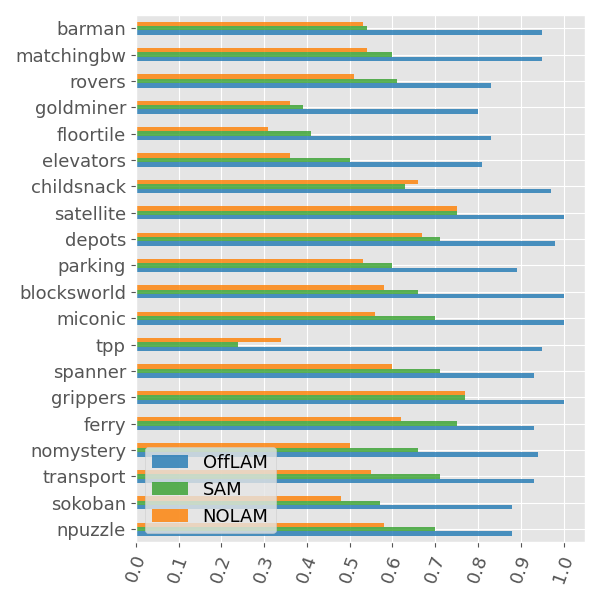
\includegraphics[width=\textwidth]{figures/10_traces_mini/syn_precision.png}
%     \caption{Syntactic precision}
%   \end{subfigure}
%   \\
%   % \begin{subfigure}[b]{0.24\textwidth}
%   %   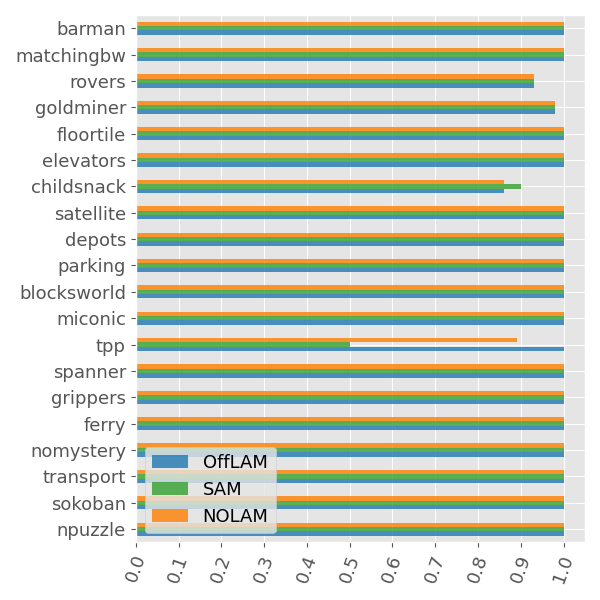
\includegraphics[width=\textwidth]{figures/10_traces_mini/syn_recall.png}
%   %   \caption{Syntactic recall}
%   % \end{subfigure}
%   \begin{subfigure}[b]{0.6\columnwidth}
%     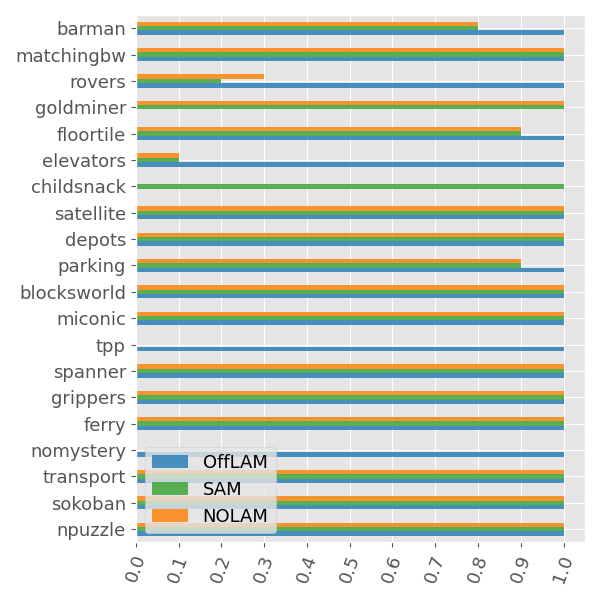
\includegraphics[width=\textwidth]{figures/10_traces_mini/solving.png}
%     \caption{Problem solving ratio}
%   \end{subfigure}
%   \\
%   \begin{subfigure}[b]{0.6\columnwidth}
%     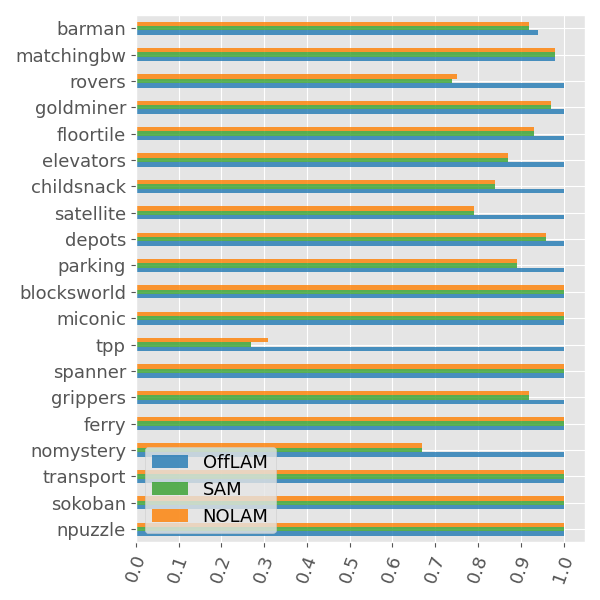
\includegraphics[width=\textwidth]{figures/10_traces_mini/app_recall.png}
%     \caption{Applicability recall}
%   \end{subfigure}




%   \caption{Evaluation metrics when learning from a training set $\Ttrain$ with $10$ traces for every domain.}
%   \label{fig:exp-mini}
% \end{figure} 


% OPTION B

\begin{figure}[ht]
% \label{fix:exp-results}
  \centering

  \begin{subfigure}[b]{\columnwidth}
    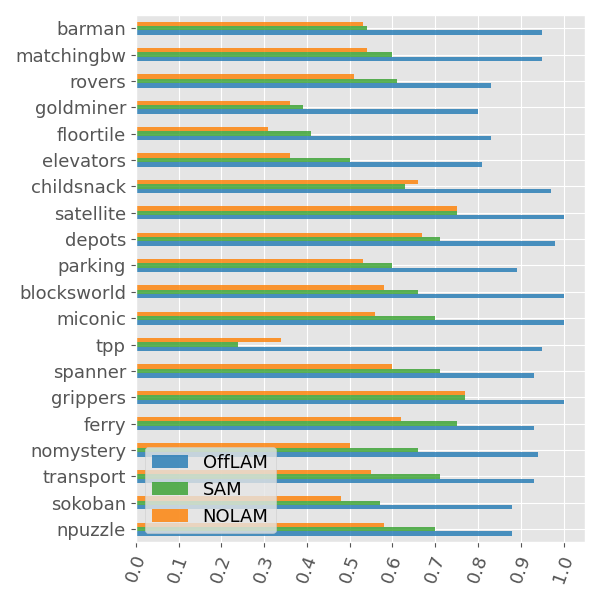
\includegraphics[width=\textwidth]{figures/10_traces_mini/syn_precision.png}
    \caption{Preconditions syntactic precision}
    \label{fig:syn-precision}
  \end{subfigure}
  \hfill
  % \begin{subfigure}[b]{0.24\textwidth}
  %   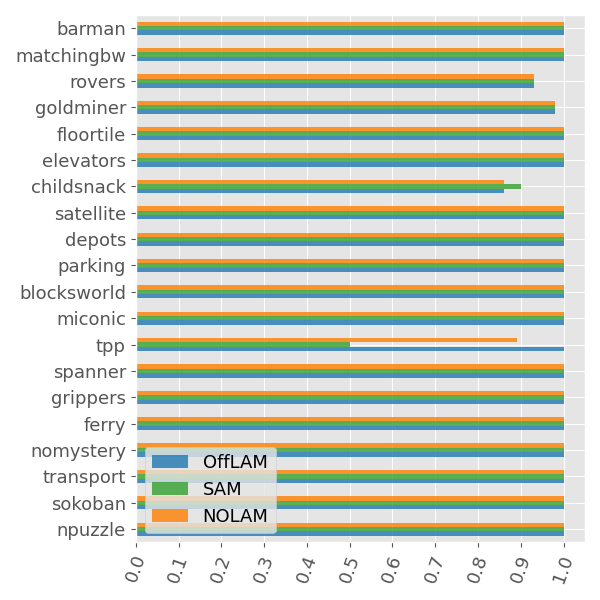
\includegraphics[width=\textwidth]{figures/10_traces_mini/syn_recall.png}
  %   \caption{Syntactic recall}
  % \end{subfigure}
  \begin{subfigure}[b]{\columnwidth}
    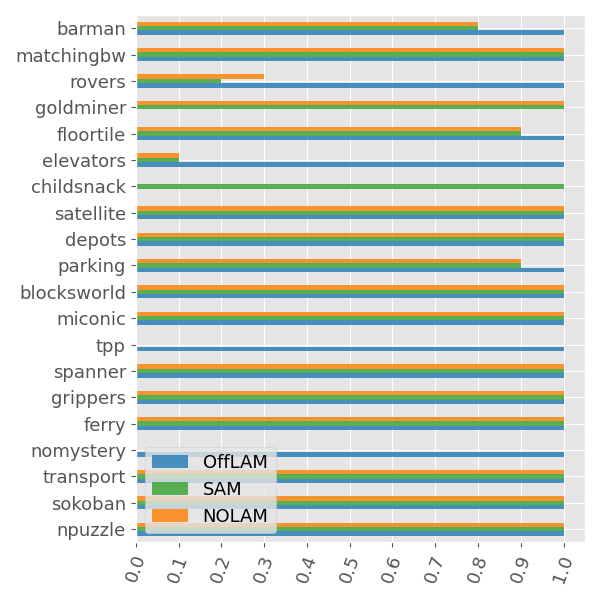
\includegraphics[width=\textwidth]{figures/10_traces_mini/solving.png}
    \caption{Problem solving ratio}
    \label{fig:solving-ratio}
  \end{subfigure}
  \hfill
  \begin{subfigure}[b]{\columnwidth}
    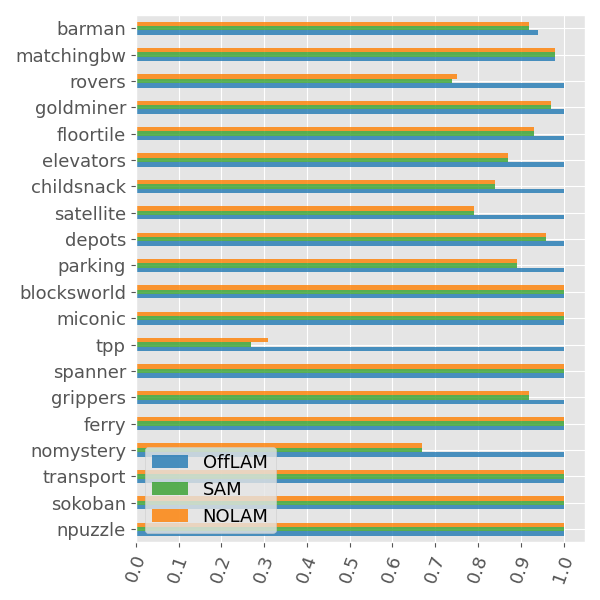
\includegraphics[width=\textwidth]{figures/10_traces_mini/app_recall.png}
    \caption{Applicability recall}
  \end{subfigure}




  \caption{Evaluation metrics for the models learned by \samshort{}, \offlam{} and \nolam{} from a training set $\Ttrain$ of $10$ traces for every domain.}
  \label{fig:exp-mini}
\end{figure} 

% \roni{Writing standard: we show here 3 concrete algorithms, not 3 approaches.}

To demonstrate our evaluation process, we used it to evaluate three state-of-the-art domain model learning algorithms, namely \samshort~\citep{juba2021safe}, \offlam~\citep{LAMANNA2025104256}, and \nolam~\citep{Lamanna24}. The results of our evaluation are described below. Due to space constraints, only a subset of the results are shown in Figure~\ref{fig:exp-mini}. All the experiments were run on a CPU Apple M1 Pro with 16 GB of RAM.
%We evaluated the learning algorithms on standard benchmark domains using the proposed metrics. 





\miniparagraph{Syntactic similarity} 
% We report syntactic precision and recall using the \emph{simple} aggregation across the preconditions and effects of all actions. \roni{It was written here that we use the cumulative aggregation and not the average here. But, this is a syntactic similarity metric, you can only aggregate over actions. Commenting this out}
Both \samshort{} and \nolam{} exhibited relatively low precondition precision ($<0.8$) across all domains, as they assume the presence of negative preconditions and include them in the learned domains. 
In contrast, \offlam{} assumes that domains do not include negative preconditions, which is a correct assumption for our benchmarks, leading to higher precision values.
In terms of precondition recall, \samshort{}'s low values stemmed from its inability to learn some actions entirely, i.e., the actions have all the preconditions and no effects, while \offlam{} and \nolam{} struggled to learn specific predicates due to domain inconsistencies (e.g., in \textsc{rovers}) or the presence of constants not bound to action parameters (e.g., in \textsc{childsnack}).
% \roni{All this discusses preconditions. What about the syntactic similarity of effects?}
% \leo{
In terms of effects, both \offlam{} and \nolam obtained syntactic precision and recall of $1$ in all domains except \textsc{rovers} (because of inconsistent effects), \textsc{goldminer} (because of an unobserved negative effect), and \textsc{childsnack} (for an unobserved positive effect). \samshort{} achieved effects the same results except for \textsc{tpp}, where it only achieved 50\% recall.
% for both positive and negative effects.} do we separate the two types in our evaluation?
% However, the domains used in the experiments do not include negative preconditions. 
% This is due to additional preconditions, as both algorithms include negative preconditions in the learned domains, which are always absent in the reference domains. For instance, in the \textsc{blocksworld} domain, the lifted action \textsc{pick\_up}$(x)$ for a block $x$ has the precondition $\textit{handempty}()$, which implies $\textit{holding}(x)$ is false. 
% % However, the domains learned by \samshort{} and \nolam{} include such negative preconditions, which lowers their syntactic precision. 
% In contrast, \offlam{} assumes domains do not include negative preconditions, resulting in more concise domains and higher precision. However, this metric's sensitivity to such additions is a limitation, as it can penalize the inclusion of predicates that implicitly hold true in the domain. 
% Regarding the aggragated recall \roni{recall of preconditions or effects?} \argaman{The metric is calculated as a combination of the two.}, all algorithms performed similarly, with perfect recall in all but four domains -- \textsc{tpp}, \textsc{childsnack}, \textsc{goldminer} and \textsc{rovers}.
% The lower recall in those domains mainly stem from missing effects.
% A prominent example is \textsc{tpp} domain, with \samshort{} having the lowest recall (i.e., $0.5$). 
% This is due to its assumption that actions cannot be executed with the same object bound to multiple parameters—an assumption that does not hold in this domain.\footnote{This is referred to as the \textit{injective binding assumption} in the \sam learning paper.} 
% The ESAM algorithm remedies this limitation~\citep{juba2021safe}.
% % In \textsc{childsnack} domain, \offlam and \nolam both 
% \roni{This explains why SAM did not work well, but what about the other algorithms? what is unique in these domains. If we do not know, that is also Ok, this is not a paper that is intended to explain the algorithms just show the benchmark}
% \leo{In \textsc{childsnack}, both \offlam{} and \nolam{} misses a positive precondition of action $put\_on\_tray$ involving a constant $kitchen$, since they do not support constants. On the opposite, \samshort{} do support constants. In \textsc{rovers}, all approaches cannot learn some positive and negative effects; indeed the IPC version of \textsc{rover} contains some inconsistent effects. In \textsc{gold-miner}, all approaches do not learn a negative effect because it is never observed in the trajectories.}



\miniparagraph{Predicted applicability} 
By design, \samshort{} and \offlam{} initially assume the preconditions of each lifted action to be the set of all possible preconditions, and remove unnecessary preconditions that are not consistent with the input trajectories, resulting in perfect applicability precision. Notably, \nolam{} achieves perfect applicability precision even without such an assumption.
The only outlier is the \textsc{childsnack} domain, where both \nolam{} and \offlam{} have a slight decrease in the precision due to the constant in the domains (which is not supported by these algorithms).
% in the precision due to $put\_on\_tray$'s precondition involving $kitchen$.
% This results from the domain including a constant -- $kitchen$ -- in a predicate of the action $put\_on\_tray$'s preconditions. 
% Indeed, this constant is not part of the action's parameters, which causes it not to be learned.
% \roni{Not clear. Do you mean NOLAM and Offlam do not support constants and SAM does?}\leo{Yes, I added a comment about this in the previous paragraph}
\offlam{} achieved the best performance in terms of applicability recall with perfect recall values in all domains except \textsc{barman}, which had a slight decrease in its recall due to a single literal miss-classified as a precondition. 
% \leo{with only a slight decrease in its recall value due to a false positive precondition for action $empty\_shot$. This results from \offlam{} assuming no negative preconditions, which prevents it from learning unnecessary ones.}
% allows to remove redundant ones with less observations than \samshort{} and \nolam{} that assume the existence of negative preconditions as well. 
Notably, the unnecessary negative preconditions learned by \samshort{} and \nolam{} only significantly impacted the recall for the \textsc{tpp} domain; indeed, all other domains had applicability recall values exceeding $0.6$. 


\miniparagraph{Predicted effects} 
% Across all domains, all algorithms achieved perfect precision and recall. This is attributed to the fact that each action in the trace dataset was observed at least once, ensuring that all effects present in the training trajectories were successfully learned.\roni{Not convincing. Observing once is not enough.}
All algorithms achieved perfect precision and recall across all domains. 
By design, \samshort{} and \offlam{} provides effects syntactic precision equal to $1$ (this also holds for \nolam{} as the trajectories are un-noisy and fully observable), since an action's effect is learned only when a literal becomes true/false after observing such action execution in some trajectory transition. This prevents \samshort{} and \offlam{} from learning unnecessary effects, hence making the false positives for the predicted effects equal to $0$, and the precision equal to $1$. 
Furthermore, the predicted effects only consider actions applicable according to the learned domain and real environment, and every lifted action execution is observed at least once in the set of trajectories. Therefore, evaluating the actions is only performed when the actions are applicable according to the learned domain. Thus, resulting in states that were already observed in the train trajectories.
% Other approaches that are less conservative than our tested algorithms might perform a different approach to learning the effects, resulting in different predictive values. 
Other, less conservative approaches may follow different effect-learning strategies, potentially leading to different precision and recall outcomes.

% when evaluating the predicted effects of an action
% $a$ in a state $s$, there is a trajectory state which satisfies the precondition of $a$ as $s$ does (otherwise $a$ would not be applicable in $s$), and thus if a literal does not change after executing $a$ in such trajectory state, then either the literal is not an effect of $a$ or it is both an effect and a precondition of $a$, which already holds in $s$ (e.g. a positive effect which is already true in $s$). Hence FN equals $0$ and the predicted effects recall equals $1$.
% precision equals 1 because of the effects syntactic precision being equal to 1 and the preconditions being a superset of the real preconditions: no false effects implies no `false changes` in the destination state reached after executing an applicable action. 



\miniparagraph{Problem-solving} 
\offlam{} achieved the highest problem-solving ratio across all domains except for \textsc{childsnack} and \textsc{goldminer}. Notably, in the \textsc{nomystery} and \textsc{tpp} domains, it is the only algorithm to produce a model capable of solving the entire test set.
In the \textsc{elevators} and \textsc{rovers} domains it highly outperforms both \samshort{} and \nolam{} with 85\% and 70\% increase in the 
solving rates respectively.
The difficulty in solving problems for \samshort{} and \nolam{} is mainly due to the learned domains having unnecessary negative preconditions. 
% Specifically, in these domains, the actions had high arity which resulted in many negative preconditions that were created for them (see Table~\ref{tab:domains} for reference). 
In \textsc{childsnack}, both \offlam{} and \nolam{} produced inapplicable plans due to the missing precondition involving the unsupported constant.
% of $put\_on\_tray$ involving the unsupported constant $kitchen$. 
% This results from the domain having a constant that was not properly learned by these algorithm which was part of the action $put\_on\_tray$'s preconditions.
% An exception is the \textsc{childsnack} domain, which includes a constant unsupported by both NOLAM and OffLAM. 
% \roni{Repetition of the sentence above?}\leo{yes, removed}
% Although plans were generated, they were deemed inapplicable, as shown in Figure~\ref{fig:false-positive-plans}.
Similarly, the plans produced with the models learned by \offlam{} are inapplicable due to a missing negative effect, which affects the precondition of subsequent plan actions.
% $(not\; (gold\_at\; ?y))$ of action $fire\_laser$, which affects the precondition of subsequent plan actions.
% We also observed that in the \textsc{goldminer} all of the plans generated using the domains \offlam learned were deemed inapplicable. This resulted from \offlam not learning the effect $(not\; (gold\_at\; ?y))$ which was crucial to the consistency of the resulting plans. 
% Because 
Such an effect was never observed in the input trajectories. Interestingly, \sam and \nolam, learned the unobserved negative effect as a negative precondition, which allows computing valid plans.


\begin{table}[b!]
\resizebox{\columnwidth}{!}{
\addtolength{\tabcolsep}{-0.4em}
\begin{tabular}{l|l|l|l|l|l|l}
% \toprule
\hline
Domain & \multicolumn{2}{c|}{Syntactic} & \multicolumn{2}{c|}{Applicability} & Solv. \% $\uparrow$ & False \% $\downarrow$ \\
 & \makecell[c]{P$\uparrow$} & \makecell[c]{R$\uparrow$} & \makecell[c]{P$\uparrow$} & \makecell[c]{R$\uparrow$} &  & \\
% \midrule
\hline
barman  & 0.95 $^{2}$ & 1.00 $^{1,2,3}$ & 1.00 $^{1,2,3}$ & 0.94 $^{2}$ & 1.00 $^{2}$ & 0.00 $^{1,2,3}$ \\
blocksworld  & 1.00 $^{2}$ & 1.00 $^{1,2,3}$ & 1.00 $^{1,2,3}$ & 1.00 $^{1,2,3}$ & 1.00 $^{1,2,3}$ & 0.00 $^{1,2,3}$ \\
childsnack & 0.97 $^{2}$ & 0.90 $^{1}$ & 1.00 $^{1}$ & 1.00 $^{2}$ & 1.00 $^{1}$ & 0.00 $^{1}$ \\
depots  & 0.98 $^{2}$ & 1.00 $^{1,2,3}$ & 1.00 $^{1,2,3}$ & 1.00 $^{2}$ & 1.00 $^{1,2,3}$ & 0.00 $^{1,2,3}$ \\
elevators  & 0.81 $^{2}$ & 1.00 $^{1,2,3}$ & 1.00 $^{1,2,3}$ & 1.00 $^{2}$ & 1.00 $^{2}$ & 0.00 $^{1,2,3}$ \\
ferry  & 0.93 $^{2}$ & 1.00 $^{1,2,3}$ & 1.00 $^{1,2,3}$ & 1.00 $^{1,2,3}$ & 1.00 $^{1,2,3}$ & 0.00 $^{1,2,3}$ \\
floortile & 0.83 $^{2}$ & 1.00 $^{1,2,3}$ & 1.00 $^{1,2,3}$ & 1.00 $^{2}$ & 1.00 $^{2}$ & 0.00 $^{1,2,3}$ \\
goldminer & 0.8 $^{2}$ & 0.98 $^{1,2,3}$ & 1.00 $^{1,2,3}$ & 1.00 $^{2}$ & 1.00 $^{1,3}$ & 0.00 $^{1,3}$ \\
grippers & 1.00 $^{2}$ & 1.00 $^{1,2,3}$ & 1.00 $^{1,2,3}$ & 1.00 $^{2}$ & 1.00 $^{1,2,3}$ & 0.00 $^{1,2,3}$ \\
matchingbw & 0.95 $^{2}$ & 1.00 $^{1,2,3}$ & 1.00 $^{1,2,3}$ & 0.98 $^{1,2,3}$ & 1.00 $^{1,2,3}$ & 0.00 $^{1,2,3}$ \\
miconic & 1.00 $^{2}$ & 1.00 $^{1,2,3}$ & 1.00 $^{1,2,3}$ & 1.00 $^{1,2,3}$ & 1.00 $^{1,2,3}$ & 0.00 $^{1,2,3}$ \\
nomystery & 0.94 $^{2}$ & 1.00 $^{1,2,3}$ & 1.00 $^{1,2,3}$ & 1.00 $^{2}$ & 1.00 $^{2}$ & 0.00 $^{1,2,3}$ \\
npuzzle & 0.88 $^{2}$ & 1.00 $^{1,2,3}$ & 1.00 $^{1,2,3}$ & 1.00 $^{1,2,3}$ & 1.00 $^{1,2,3}$ & 0.00 $^{1,2,3}$ \\
parking & 0.89 $^{2}$ & 1.00 $^{1,2,3}$ & 1.00 $^{1,2,3}$ & 1.00 $^{2}$ & 1.00 $^{2}$ & 0.00 $^{1,2,3}$ \\
rovers & 0.83 $^{2}$ & 0.93 $^{1,2,3}$ & 1.00 $^{1,2,3}$ & 1.00 $^{2}$ & 1.00 $^{2}$ & 0.00 $^{1,2,3}$ \\
satellite & 1.00 $^{2}$ & 1.00 $^{1,2,3}$ & 1.00 $^{1,2,3}$ & 1.00 $^{2}$ & 1.00 $^{1,2,3}$ & 0.00 $^{1,2,3}$ \\
sokoban & 0.88 $^{2}$ & 1.00 $^{1,2,3}$ & 1.00 $^{1,2,3}$ & 1.00 $^{1,2,3}$ & 1.00 $^{1,2,3}$ & 0.00 $^{1,2,3}$ \\
spanner & 0.93 $^{2}$ & 1.00 $^{1,2,3}$ & 1.00 $^{1,2,3}$ & 1.00 $^{1,2,3}$ & 1.00 $^{1,2,3}$ & 0.00 $^{1,2,3}$ \\
tpp & 0.95 $^{2}$ & 1.00 $^{2}$ & 1.00 $^{1,2,3}$ & 1.00 $^{2}$ & 1.00 $^{2}$ & 0.00 $^{1,2,3}$ \\
transport & 0.93 $^{2}$ & 1.00 $^{1,2,3}$ & 1.00 $^{1,2,3}$ & 1.00 $^{1,2,3}$ & 1.00 $^{1,2,3}$ & 0.00 $^{1,2,3}$ \\
% \bottomrule
\hline
\end{tabular}
}
\caption{Best metric values for every domain obtained among \sam, \offlam, \nolam, respectively denoted by 1,2, and 3; P indicates the precision and R the recall, $\uparrow$ (resp. $\downarrow$) denotes the higher (resp. lower) the better. The predicted effects precision and recall equal $1$ for all approaches in all domains.}
\label{tab:best}
\end{table}




% \hline
% barman  & 0.95 $^{2}$ & 1.00 $^{1,2,3}$ & 1 $^{1,2,3}$ & 0.94 $^{2}$ & 1 $^{2}$ & 0 $^{1,2,3}$ \\
% blocksworld  & 1 $^{2}$ & 1 $^{1,2,3}$ & 1 $^{1,2,3}$ & 1 $^{1,2,3}$ & 1 $^{1,2,3}$ & 0 $^{1,2,3}$ \\
% childsnack & 0.97 $^{2}$ & 0.9 $^{1}$ & 1 $^{1}$ & 1 $^{2}$ & 1 $^{1}$ & 0 $^{1}$ \\
% depots  & 0.98 $^{2}$ & 1 $^{1,2,3}$ & 1 $^{1,2,3}$ & 1 $^{2}$ & 1 $^{1,2,3}$ & 0 $^{1,2,3}$ \\
% elevators  & 0.81 $^{2}$ & 1 $^{1,2,3}$ & 1 $^{1,2,3}$ & 1 $^{2}$ & 1 $^{2}$ & 0 $^{1,2,3}$ \\
% ferry  & 0.93 $^{2}$ & 1 $^{1,2,3}$ & 1 $^{1,2,3}$ & 1 $^{1,2,3}$ & 1 $^{1,2,3}$ & 0 $^{1,2,3}$ \\
% floortile & 0.83 $^{2}$ & 1 $^{1,2,3}$ & 1 $^{1,2,3}$ & 1 $^{2}$ & 1 $^{2}$ & 0 $^{1,2,3}$ \\
% goldminer & 0.8 $^{2}$ & 0.98 $^{1,2,3}$ & 1 $^{1,2,3}$ & 1 $^{2}$ & 1 $^{1,3}$ & 0 $^{1,3}$ \\
% grippers & 1 $^{2}$ & 1 $^{1,2,3}$ & 1 $^{1,2,3}$ & 1 $^{2}$ & 1 $^{1,2,3}$ & 0 $^{1,2,3}$ \\
% matchingbw & 0.95 $^{2}$ & 1 $^{1,2,3}$ & 1 $^{1,2,3}$ & 0.98 $^{1,2,3}$ & 1 $^{1,2,3}$ & 0 $^{1,2,3}$ \\
% miconic & 1 $^{2}$ & 1 $^{1,2,3}$ & 1 $^{1,2,3}$ & 1 $^{1,2,3}$ & 1 $^{1,2,3}$ & 0 $^{1,2,3}$ \\
% nomystery & 0.94 $^{2}$ & 1 $^{1,2,3}$ & 1 $^{1,2,3}$ & 1 $^{2}$ & 1 $^{2}$ & 0 $^{1,2,3}$ \\
% npuzzle & 0.88 $^{2}$ & 1 $^{1,2,3}$ & 1 $^{1,2,3}$ & 1 $^{1,2,3}$ & 1 $^{1,2,3}$ & 0 $^{1,2,3}$ \\
% parking & 0.89 $^{2}$ & 1 $^{1,2,3}$ & 1 $^{1,2,3}$ & 1 $^{2}$ & 1 $^{2}$ & 0 $^{1,2,3}$ \\
% rovers & 0.83 $^{2}$ & 0.93 $^{1,2,3}$ & 1 $^{1,2,3}$ & 1 $^{2}$ & 1 $^{2}$ & 0 $^{1,2,3}$ \\
% satellite & 1 $^{2}$ & 1 $^{1,2,3}$ & 1 $^{1,2,3}$ & 1 $^{2}$ & 1 $^{1,2,3}$ & 0 $^{1,2,3}$ \\
% sokoban & 0.88 $^{2}$ & 1 $^{1,2,3}$ & 1 $^{1,2,3}$ & 1 $^{1,2,3}$ & 1 $^{1,2,3}$ & 0 $^{1,2,3}$ \\
% spanner & 0.93 $^{2}$ & 1 $^{1,2,3}$ & 1 $^{1,2,3}$ & 1 $^{1,2,3}$ & 1 $^{1,2,3}$ & 0 $^{1,2,3}$ \\
% tpp & 0.95 $^{2}$ & 1 $^{2}$ & 1 $^{1,2,3}$ & 1 $^{2}$ & 1 $^{2}$ & 0 $^{1,2,3}$ \\
% transport & 0.93 $^{2}$ & 1 $^{1,2,3}$ & 1 $^{1,2,3}$ & 1 $^{1,2,3}$ & 1 $^{1,2,3}$ & 0 $^{1,2,3}$ \\
% % \bottomrule
% \hline

% \roni{Important: Can we add to the domains table the columns: Constants (Const.), Injective binding (Inj. Bind), and Negative preconditions (Neg. Pre.)? this will connect to the reults we observed.}
% \leo{added. I am not sure about the injective binding assumption since even though an action can take as input objects of the same type, then the fact that it (can) actually involves the same object multiple times depends on the domain and traces. I am not sure this is easily deducible from the action signature only, as I currently did}


% \roni{The results are Ok. Perhaps would be good to add a summary paragraph that says something like As the results show, different algorithms work well in different domains and for different metrics. }
% \leo{I wrote a draft for this }

% \leo{
\miniparagraph{Results summary} 
Table \ref{tab:best} lists the best performance for each metric and domain on the proposed benchmark. The superscripts in each cell indicate which of the evaluated algorithms --- \sam{}, \offlam{}, and \nolam{} --- obtained the best performance in this metric and domain. As the results show, while the algorithms are able to reach impressive performance in our benchmark, one can see that different algorithms perform better in different domains and for different metrics. 
For example, \offlam{} provides better syntactic precondition precision than \samshort{} and \nolam{} in all domains. However, it fails to solve some test problems in \textsc{goldminer} since it does not learn negative effects (while \sam and \offlam{} can learn them). 
% are not learned, as in \textsc{goldminer} domain; while this is not the case for \samshort{} and \nolam{}. 
Indeed, the syntactic precision performance gap between \offlam{} and other approaches (Figure \ref{fig:syn-precision}) is not reflected in terms of problem-solving (Figure \ref{fig:solving-ratio}) as, e.g., in domain \textsc{matchingbw}. 
This provides empirical evidence of the drawbacks in syntactic similarity discussed in Section \ref{sec:problem-setting}.
Interestingly, the different approaches to deal with action objects binding can significantly impact the performance in domains where the injective action binding assumption is violated, as in \textsc{elevators} and \textsc{tpp}.  


% BACKUP IF I DO DAMAGE
% We assessed the best performance of three state-of-the-art approaches on the proposed benchmark (Table \ref{tab:best}). As the results show, different algorithms perform better in different domains and for different metrics. On the one hand, \offlam{} provides better syntactic precision than \samshort{} and \nolam{}, on the other hand, it assumes there are no negative preconditions, which can degrade problem-solvability performance when some negative effects are not learned, as in \textsc{goldminer} domain; while this is not the case for \samshort{} and \nolam{}. 
% Moreover, the syntactic precision performance gap between \offlam{} and other approaches (Figure \ref{fig:syn-precision}) is not reflected in terms of problem-solving (Figure \ref{fig:solving-ratio}) as, e.g., in domain \textsc{matchingbw}. This provides empirical evidence of the drawbacks in syntactic similarity discussed in Section \ref{sec:problem-setting}.
% Interestingly, the different approaches to deal with action objects binding can significantly impact the performance in domains where the injective action binding assumption is violated, as in \textsc{elevators} and \textsc{tpp}.  
